\documentclass{labreport}

\usepackage{amsmath}
\usepackage{tikz}
\usepackage{caption}
\usepackage{mathtools}
\usepackage{subcaption}
\usepackage{csquotes}
\usepackage{dirtytalk}

\title{Оценка поведения многокаскадного усилителя, охваченного обратными связами}
\subtitle{по домашней работе № 2}
\author{И.В. Бобренко}
\group{ИУ6-42Б}
\descipline{Электроника}

\newcommand{\Iclx}[1]{I'_{#1} + jI''_{#1}}
\newcommand{\uin}{u_\text{вх}}
\newcommand{\uout}{u_\text{вых}}
\newcommand{\uind}{\frac{d\uin(\tau)}{d\tau}}

\newcommand{\fT}[1]{\frac{#1T}{2}}

% \titleformat{\chapter}[display]{\Huge\bfseries}{}{0pt}{\Huge\bfseries}

\begin{document}

\maketitle


\chapter{Задание}

\textbf{Вариант 35}

Найти в схеме все обратные связи и дать им определение. Что произойдёт с коэффициентами передачи усилителя $K_\text{uoc}$ и $K_\text{ioc}$, если разомкнуть цепь общей ОС?

\begin{figure}[h]
    \centering
    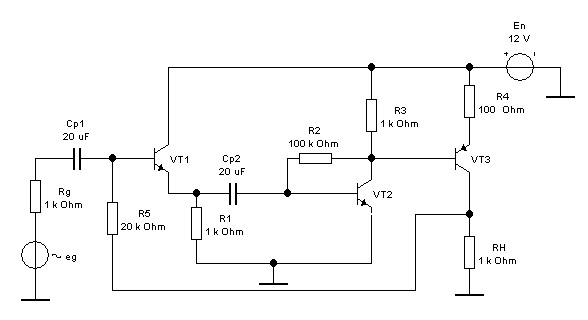
\includegraphics[width=\linewidth]{ek_task2.jpg}
    \caption{Схема каскадов}
    \label{fig:my_label}
\end{figure}

\section{Решение связей}
\subsection{Первый каскад (VT1)}
К каскаду относятся:
\begin{itemize}
    \item $R_1$ -- Резистор последовательной ООС по напряжению и нагрузка первого каскада.
\end{itemize}


\subsection{Второй каскад (VT2)}
К каскаду относятся:
\begin{itemize}
    \item $R_2$ -- Резистор параллельной ООС по напряжению
    \item $R_3$ -- Задание тока смещения на VT2
\end{itemize}

\subsection{Третий каскад (VT3)}
К каскаду относятся:
\begin{itemize}
    \item $R_3$ -- Резистор последовательной ООС по току
    \item $R_4$ -- Резистор последовательной ООС по току и задание тока смещения на VT3
    \item $R_n$ -- Нагрузка третьего каскада
\end{itemize}


\subsection{Общая связь}
К общей связи относятся:
\begin{itemize}
    \item $R_4$ -- Резистор последовательной ООС по напряжению
    
\end{itemize}



Из схемы очевидно, что цепь обратной связи подключена параллельно входной и выходной цепи усилителя, за счет чего образуется параллельная обратная связь по напяржению. 
Таким образом, общая обратная связь является параллельной ООС по напряжению. 

\section{Коэффициенты}

Коэффициент усиления по напряжению:
\begin{gather*}
    K_\text{uoc} = \frac{K_u}{1+K_u\cdot b}
\end{gather*}

Коэффициент усиления по току:
\begin{gather*}
    K_\text{ioc} = \frac{K_i}{1+K_i\cdot b}
\end{gather*}

Где $b$ -- коэффициент передачи цепи обратной связи. Очевидно, что если обратная связь размыкается, то коэффициент усиления по напряжению и току увеличивается.

\say{Коэффициент усиления при замкнутой цепи обратной связи никогда не может стать больше, чем коэффициент усиления при разомкнутой цепи обратной связи.} -- Искусство схемотехники.

\chapter{Выводы}
\begin{itemize}
  \item   Первый каскад -- \textbf{последовательная ООС по напряжению}.

\item  Пассивные элементы обратной связи первого каскада: $R_1$.

\item Второй каскад -- \textbf{параллельная ООС по напряжению}.

\item Пассивные элементы обратной связи второго каскада: $R_2$.

\item Третий каскад -- \textbf{последовательная ООС по току}.

\item Пассивные элементы обратной связи третьего каскада: $R_3$, $R_4$.

\item Общая обратная связь -- \textbf{параллельная ООС по напряжению}.

\item Пассивные элементы обратной связи первого каскада: $R_5$.

\item При размыкании ООС, коэффициент усиления по напряжению \textbf{увеличится}.

\item При размыкании ООС, коэффициент усиления по току \textbf{увеличится}.

\item При введении ООС, параметры усилителя изменятся \textbf{в глубину обратной связи раз}. 
\end{itemize}

\section{Сипсок использованных источников:}

\begin{itemize}
    \item Электроника -- О. В. Миловзоров, И. Г. Панков
    \item Электронные устройства автоматики -- Г. В. Королев
    \item Искусство схемотехники -- П. Хоровиц, У. Хилл
\end{itemize}
    
\end{document}